\section{Phần dịch trang 20 đến 30}
Số lẻ: 128

Giải pháp cho vấn đề này là lưu trữ số nguyên được chọn ngẫu nhiên vào một biến và chỉ gọi lại \texttt{nextInt} khi thực sự cần một số ngẫu nhiên khác. Đoạn mã sau đây thực hiện tác vụ này:

\begin{verbatim}
// đoạn mã này hoạt động chính xác
Random r = new Random();
int n = r.nextInt(); // lưu số ngẫu nhiên vào một biến
if (n % 2 == 0) {
    System.out.println("Even number: " + n);
} else {
    System.out.println("Odd number: " + n);
}
\end{verbatim}

\subsection*{Mô phỏng (Simulations)}

Khoa học và kỹ thuật truyền thống đòi hỏi nhiều sự tương tác trong thế giới thực. Các nhà khoa học tiến hành thực nghiệm để kiểm tra các giả thuyết của họ và các kỹ sư xây dựng các mẫu thử (prototypes) để thử nghiệm các thiết kế của mình. Nhưng ngày càng có nhiều nhà khoa học và kỹ sư tìm đến máy tính như một cách để tăng năng suất bằng cách chạy các mô phỏng (simulations) trước nhằm khám phá các khả năng, trước khi họ tiến hành một thực nghiệm thực tế hoặc xây dựng một mẫu thử thực tế. Một nhà khoa học máy tính nổi tiếng tên là Jeanette Wing đã lập luận rằng việc tăng cường sử dụng tính toán này của các nhà khoa học và kỹ sư sẽ dẫn đến tư duy máy tính (computational thinking) được xem là nền tảng, giống như cách mà việc đọc, viết và làm toán được coi là nền tảng ngày nay.

Dưới góc độ lập trình, hai thành phần chính trong một mô phỏng là các số giả ngẫu nhiên (pseudorandom numbers) và các vòng lặp (loops). Một số mô phỏng có thể được viết bằng cách sử dụng vòng lặp \texttt{for}, nhưng thông thường chúng ta sử dụng vòng lặp \texttt{while} vì mô phỏng cần được chạy vô hạn cho đến khi một điều kiện nào đó được thỏa mãn.

Là một ví dụ đơn giản, chúng ta hãy xem cách mô phỏng việc tung hai con xúc xắc cho đến khi tổng số điểm của chúng bằng 7. Chúng ta có thể sử dụng một đối tượng \texttt{Random} để mô phỏng các con xúc xắc, gọi nó một lần cho mỗi con xúc xắc. Chúng ta muốn lặp lại cho đến khi tổng bằng 7 và có thể in ra các lần tung khác nhau xuất hiện khi chạy mô phỏng. Dưới đây là một thử nghiệm đầu tiên khá tốt:

\begin{verbatim}
Random r = new Random();
while (sum != 7) {
    // tung xúc xắc một lần
    int roll1 = r.nextInt(6) + 1;
    int roll2 = r.nextInt(6) + 1;
    int sum = roll1 + roll2;
    System.out.println(roll1 + " + " + roll2 + " = " + sum);
}
\end{verbatim}

Đoạn mã trên tạo ra lỗi trình biên dịch sau:

\begin{verbatim}
Dice.java:7: error: cannot find symbol
symbol : variable sum
location: class Dice
    while (sum != 7) {
              ^
1 error
\end{verbatim}

Vấn đề là điều kiện kiểm tra vòng lặp \texttt{while} tham chiếu đến biến \texttt{sum}, nhưng biến đó lại được khai báo bên trong thân vòng lặp. Chúng ta không thể khai báo biến trong phạm vi bên trong (inner scope) vì chúng ta cần tham chiếu đến nó trong điều kiện kiểm tra vòng lặp. Vì vậy, chúng ta phải chuyển khai báo biến lên trước vòng lặp. Chúng ta cũng phải gán cho biến một giá trị ban đầu để đảm bảo rằng nó sẽ đi vào vòng lặp. Đoạn mã này là một ví dụ khác về thời điểm chúng ta cần chuẩn bị trước cho vòng lặp (prime the loop):

\begin{verbatim}
Random r = new Random();
int sum = 0; // đặt thành 0 để đảm bảo chúng ta vào vòng lặp
while (sum != 7) {
    // tung xúc xắc một lần
    int roll1 = r.nextInt(6) + 1;
    int roll2 = r.nextInt(6) + 1;
    sum = roll1 + roll2;
    System.out.println(roll1 + " + " + roll2 + " = " + sum);
}
\end{verbatim}

Phiên bản này của đoạn mã biên dịch và hoạt động chính xác. Một kết quả chạy mẫu như sau:

\begin{verbatim}
1 + 4 = 5 
5 + 6 = 11 
1 + 3 = 4 
4 + 3 = 7 
\end{verbatim}

\subsection*{Vòng lặp do/while (do/while Loop)}

Vòng lặp \texttt{while} là vòng lặp không xác định (indefinite loop) tiêu chuẩn, nhưng Java cung cấp một số giải pháp thay thế khác. Phần này trình bày về vòng lặp \texttt{do/while}. Các biến thể khác được bao gồm trong Phụ lục C.

Như chúng ta đã thấy, vòng lặp \texttt{while} kiểm tra điều kiện ở "đỉnh" vòng lặp, trước khi nó thực thi câu lệnh mà nó kiểm soát. Java có một giải pháp thay thế được gọi là vòng lặp \texttt{do/while} kiểm tra điều kiện ở "đáy" vòng lặp. Vòng lặp \texttt{do/while} có cú pháp như sau:

\begin{verbatim}
do {
    <câu lệnh>;
    ...
    <câu lệnh>;
} while (<điều kiện>);
\end{verbatim}

Dưới đây là một số mã mẫu sử dụng vòng lặp \texttt{do/while}:

\begin{verbatim}
int number = 1;
do {
    number *= 2;
} while (number <= 200);
\end{verbatim}

Vòng lặp này tạo ra kết quả giống như vòng lặp \texttt{while} tương ứng, nhân đôi biến \texttt{number} cho đến khi giá trị của nó đạt đến 256, là lũy thừa đầu tiên của 2 lớn hơn 200. Nhưng không giống như vòng lặp \texttt{while}, vòng lặp \texttt{do/while} luôn thực thi các câu lệnh được kiểm soát của nó ít nhất một lần. Sơ đồ trong Hình 5.2 cho thấy luồng điều khiển trong một vòng lặp \texttt{do/while}.

Hình 5.2 Luồng hoạt động của vòng lặp do/while
\begin{center}
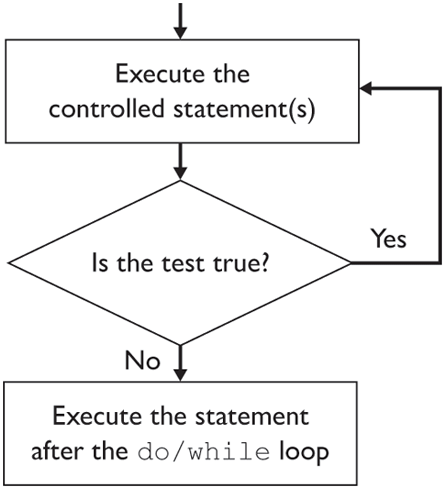
\includegraphics{Pictures/ch05_p25_img0.png}
\end{center}

Vòng lặp \texttt{do/while} hữu ích nhất trong các tình huống mà bạn biết mình phải thực thi vòng lặp ít nhất một lần. Ví dụ, trong phần trước chúng ta đã viết đoạn mã sau để mô phỏng việc tung hai con xúc xắc cho đến khi bạn có tổng bằng 7:

\begin{verbatim}
Random r = new Random();
int sum = 0; // đặt thành 0 để đảm bảo chúng ta vào vòng lặp
while (sum != 7) {
    // tung xúc xắc một lần
    int roll1 = r.nextInt(6) + 1;
    int roll2 = r.nextInt(6) + 1;
    sum = roll1 + roll2;
    System.out.println(roll1 + " + " + roll2 + " = " + sum);
}
\end{verbatim}

Chúng ta đã phải chuẩn bị trước cho vòng lặp bằng cách đặt \texttt{sum} thành 0 để máy tính đi vào vòng lặp. Với vòng lặp \texttt{do/while}, chúng ta có thể loại bỏ bước chuẩn bị này:

\begin{verbatim}
Random r = new Random();
int sum;
do {
    // tung xúc xắc một lần
    int roll1 = r.nextInt(6) + 1;
    int roll2 = r.nextInt(6) + 1;
    sum = roll1 + roll2;
    System.out.println(roll1 + " + " + roll2 + " = " + sum);
} while (sum != 7);
\end{verbatim}

Trong phiên bản này, chúng ta luôn thực thi thân vòng lặp ít nhất một lần, điều này giúp gán một giá trị cho biến \texttt{sum} trước khi nó đi tới điều kiện kiểm tra vòng lặp hiện xuất hiện ở đáy vòng lặp.

Có nhiều bài toán lập trình mà việc sử dụng vòng lặp \texttt{do/while} là phù hợp. Các vòng lặp này thường hữu ích trong các chương trình tương tác khi bạn biết mình muốn thực hiện một việc gì đó ít nhất một lần. Ví dụ: bạn có thể có một vòng lặp cho phép người dùng chơi một trò chơi nhiều lần; bạn có thể khá chắc chắn rằng người dùng sẽ muốn chơi ít nhất một lần. Tương tự như thế, nếu bạn đang chơi một trò chơi đoán số với người dùng, bạn sẽ luôn phải nhận được ít nhất một lượt đoán.

\subsection*{5.2 Thuật toán hàng rào (Fencepost Algorithms)}

Một bài toán lập trình phổ biến liên quan đến một loại vòng lặp đặc biệt được gọi là vòng lặp hàng rào (fencepost loop). Hãy xem xét bài toán sau: Bạn muốn dựng một hàng rào dài 100 yard, và bạn muốn lắp một cây cột (post) sau mỗi 10 yard. Bạn cần bao nhiêu cây cột? Nếu bạn nhẩm nhanh một phép chia trong đầu, bạn có thể nghĩ rằng mình cần 10 cây cột, nhưng thực tế bạn cần 11 cây cột. Đó là vì hàng rào bắt đầu và kết thúc bằng các cây cột. Nói cách khác, một hàng rào trông giống như Hình 5.3.

Hình 5.3 Một hàng rào điển hình

Vì bạn muốn có cột ở cả ngoài cùng bên trái và ngoài cùng bên phải, bạn không thể sử dụng vòng lặp đơn giản sau đây (nó không dựng cây cột cuối cùng):

\begin{verbatim}
for (chiều dài hàng rào) {
    dựng một cây cột.
    gắn một đoạn dây kẽm.
}
\end{verbatim}

Nếu bạn sử dụng vòng lặp trên, bạn sẽ có một hàng rào trông giống như Hình 5.4.

Hình 5.4 Một hàng rào bị lỗi

Việc thay đổi thứ tự của hai thao tác cũng không giải quyết được vấn đề, bởi vì khi đó bạn sẽ bỏ sót cây cột đầu tiên. Vấn đề với vòng lặp này là nó tạo ra số cây cột bằng đúng số đoạn dây kẽm, nhưng chúng ta biết rằng chúng ta cần thêm một cây cột nữa. Đó là lý do tại sao bài toán này đôi khi còn được gọi là bài toán "vòng lặp rưỡi" (loop and a half) — chúng ta muốn thực thi một nửa vòng lặp này (dựng một cây cột) thêm một lần nữa.